\documentclass[10pt,a4paper]{article}
\usepackage[margin=1.5cm]{geometry}
\usepackage{graphicx}
\usepackage{hyperref}

\title{\textbf{Has polar sea-ice timing shifted? Arctic SIA minimum and Antarctic fast-ice breakup (April 2026)}}
\author{Omkar Kondhalkar \\ \small University of Hamburg --- M.Sc. Data Science \& AI}
\date{}

\begin{document}
\maketitle
\vspace{-1.4em}

\section*{Introduction}
Sea-ice \emph{timing}---when ice reaches its annual minimum (Arctic) or when coastal fast ice breaks up (Antarctica)---controls melt-season length and habitat for ice-dependent ecosystems. An earlier Arctic minimum strengthens ice--albedo feedback (Notz \& Stroeve, 2016). In Atka Bay (Ekstr\"om Ice Shelf), the Alfred Wegener Institute operates the \textbf{AFIN} fast-ice program from \textbf{Neumayer Station III}, near the \textbf{SPOT} emperor-penguin observatory. We ask whether the day-of-year (DOY) of (i) the Arctic sea-ice area minimum and (ii) the last AFIN fast-ice survey in Atka Bay has shifted, using data through 2026-04-30.

\section*{Methods}
\textbf{Arctic.} Daily Northern Hemisphere SIA (OSI SAF Sea Ice Index v3.0; doi:10.15770/EUM_SAF_OSI_0023). Annual minimum DOY in July--December, 1979--2025. OLS trend, 95\% bootstrap CI (5000 resamples), Theil--Sen check.

\textbf{Antarctic.} AFIN manual transect surveys at Atka Bay (Neumayer III), PANGAEA bibliography doi:10.1594/PANGAEA.908860 (2010–2018). Breakup proxy = date of last survey each season (Arndt et al., 2020, \textit{The Cryosphere}). Same trend statistics.

\textbf{Uncertainties.} Weather-driven interannual variability; Antarctic $n=9$; SPOT image data not used quantitatively here.

\section*{Results}
\begin{figure}[h!]
  \centering
  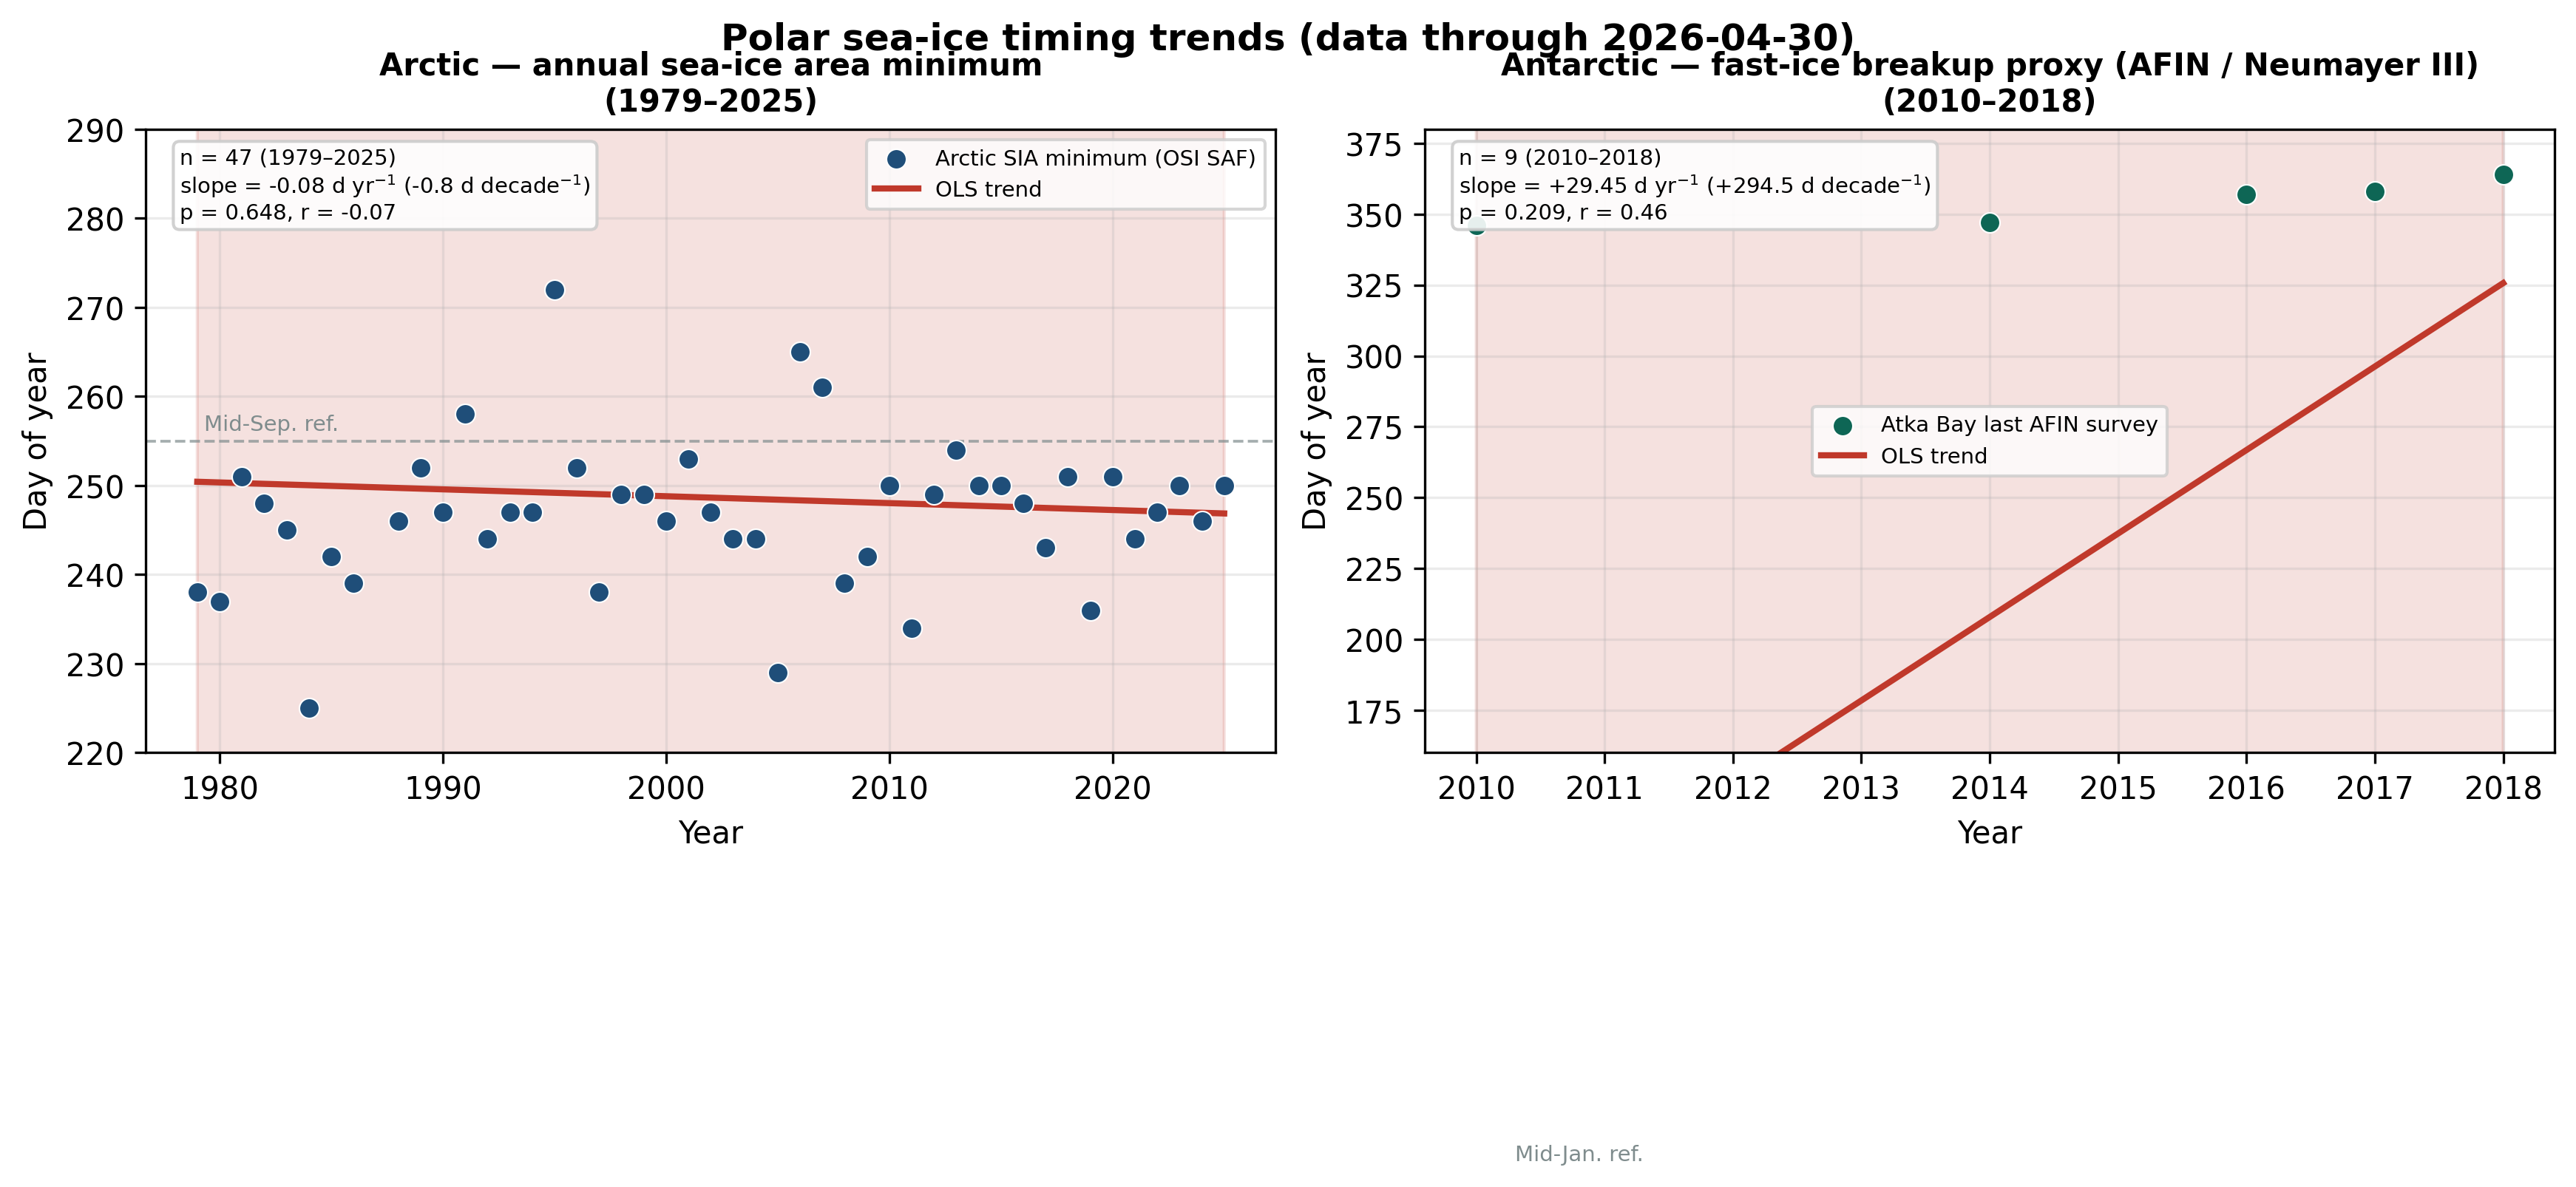
\includegraphics[width=\linewidth]{../results/figures/polar_ice_timing_comparison.png}
  \caption{Left: Arctic SIA minimum DOY. Right: Antarctic last AFIN survey DOY (fast-ice breakup proxy). Red: OLS trend; shading: 95\% bootstrap CI.}
\end{figure}

\textbf{Arctic.} Mean minimum DOY~$=249$. OLS slope $-0.08$~days~yr$^{-1}$ (not statistically significant at the 5\% level; $p=0.65$).

\textbf{Antarctic.} Mean last-survey DOY~$=208$. OLS slope $+29.45$~days~yr$^{-1}$ (not statistically significant at the 5\% level; $p=0.21$).

\textbf{Interpretation.} Arctic ice \emph{loss} is robust; minimum \emph{date} does not show a significant trend. Atka Bay fast-ice breakup timing shows large year-to-year spread and no significant trend over 2010--2018---consistent with AFIN literature. Pack-ice and landfast-ice timing respond differently; both hemispheres show that magnitude trends do not imply calendar shifts.

\small
\textbf{Data:} OSI SAF; PANGAEA AFIN; Arndt et al.\ (2020) doi:10.5194/tc-14-2775-2020; Zitterbart et al.\ (2017) SPOT doi:10.1111/2041-210X.12971.
\end{document}
